\documentclass[12pt]{article}
\usepackage{minted}
\usepackage{graphicx}
\usepackage[margin=0.25in]{geometry}

\begin{document} 
	\noindent
	Dan Jandel C. De Ramos\\
	BSCpE 2-1\\
	Made with \LaTeX \\
	\\
	Activity 2 using next()\\
	Source Code:
			
	\begin{minted}[tabsize=5]{java}         
/*
* Written by: Dan Jandel C. De Ramos
* Polytechnic University of the Philippines Biñan
* Bachelor of Science in Computer Engineering 2-1
*/

import java.util.Scanner;

public class Activity_2_n{
public static void main(String[]args){
	
	Scanner favoriteFruitScanner = new Scanner(System.in);
	String favoriteFruit;
	
	Scanner favoriteColorScanner = new Scanner(System.in);
	String favoriteColor;
	
	System.out.println();
	
	System.out.println("\u2022 Activity 2 using next() \u2022");
	
	System.out.println();
	
	System.out.println("What is your favorite fruit?");
	favoriteFruit = favoriteFruitScanner.next();    
	
	System.out.println();
	
	System.out.println("What is your favorite color?");
	favoriteColor = favoriteColorScanner.next();
	
	favoriteFruitScanner.close();
	favoriteColorScanner.close();
	
	System.out.println();        
	
	System.out.println("I wonder what a " + favoriteColor +
	" " + favoriteFruit + " would taste like");
	
	System.out.println();
	
}
}
	\end{minted}
	\clearpage
	\noindent
	Output:\\
	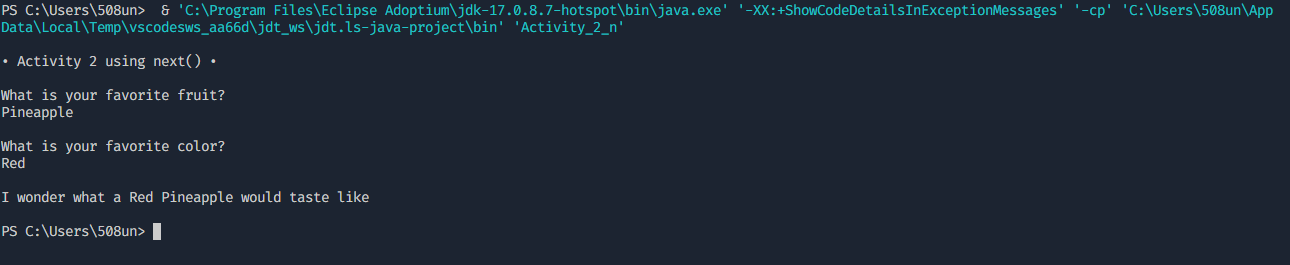
\includegraphics[width=\textwidth]{output2n}
\end{document}